\documentclass[a4paper,12pt]{jarticle}
\input ./chap01_preamble.tex
\graphicspath{%
  {../text01-img/}%
}
% !TEX root = ./chap01_03.tex
\begin{document}
\section[ラズベリーパイになれよう(2)]{ラズベリーパイになれよう(2)}
\subsection{写真をさつえいしよう}
\refstepcounter{Exercise}
\subsection{\theExercise ウェブカメラで写真をさつえいしよう}
\addtocounter{Exercise}{-1}\refstepcounter{Exercise}\label{E:webcam}
ウェブカメラを使用して画像をさつえいをします。

まずは、ラズベリーパイにウェブカメラを接続しましょう。マウスと同じように、ウェブカメラのUSBのたんしをラズベリーパイのUSBたんしへ差し込みます。



\begin{figure}[ht]
  \centering
  \begin{minipage}{8.528cm}
    {\upshape
      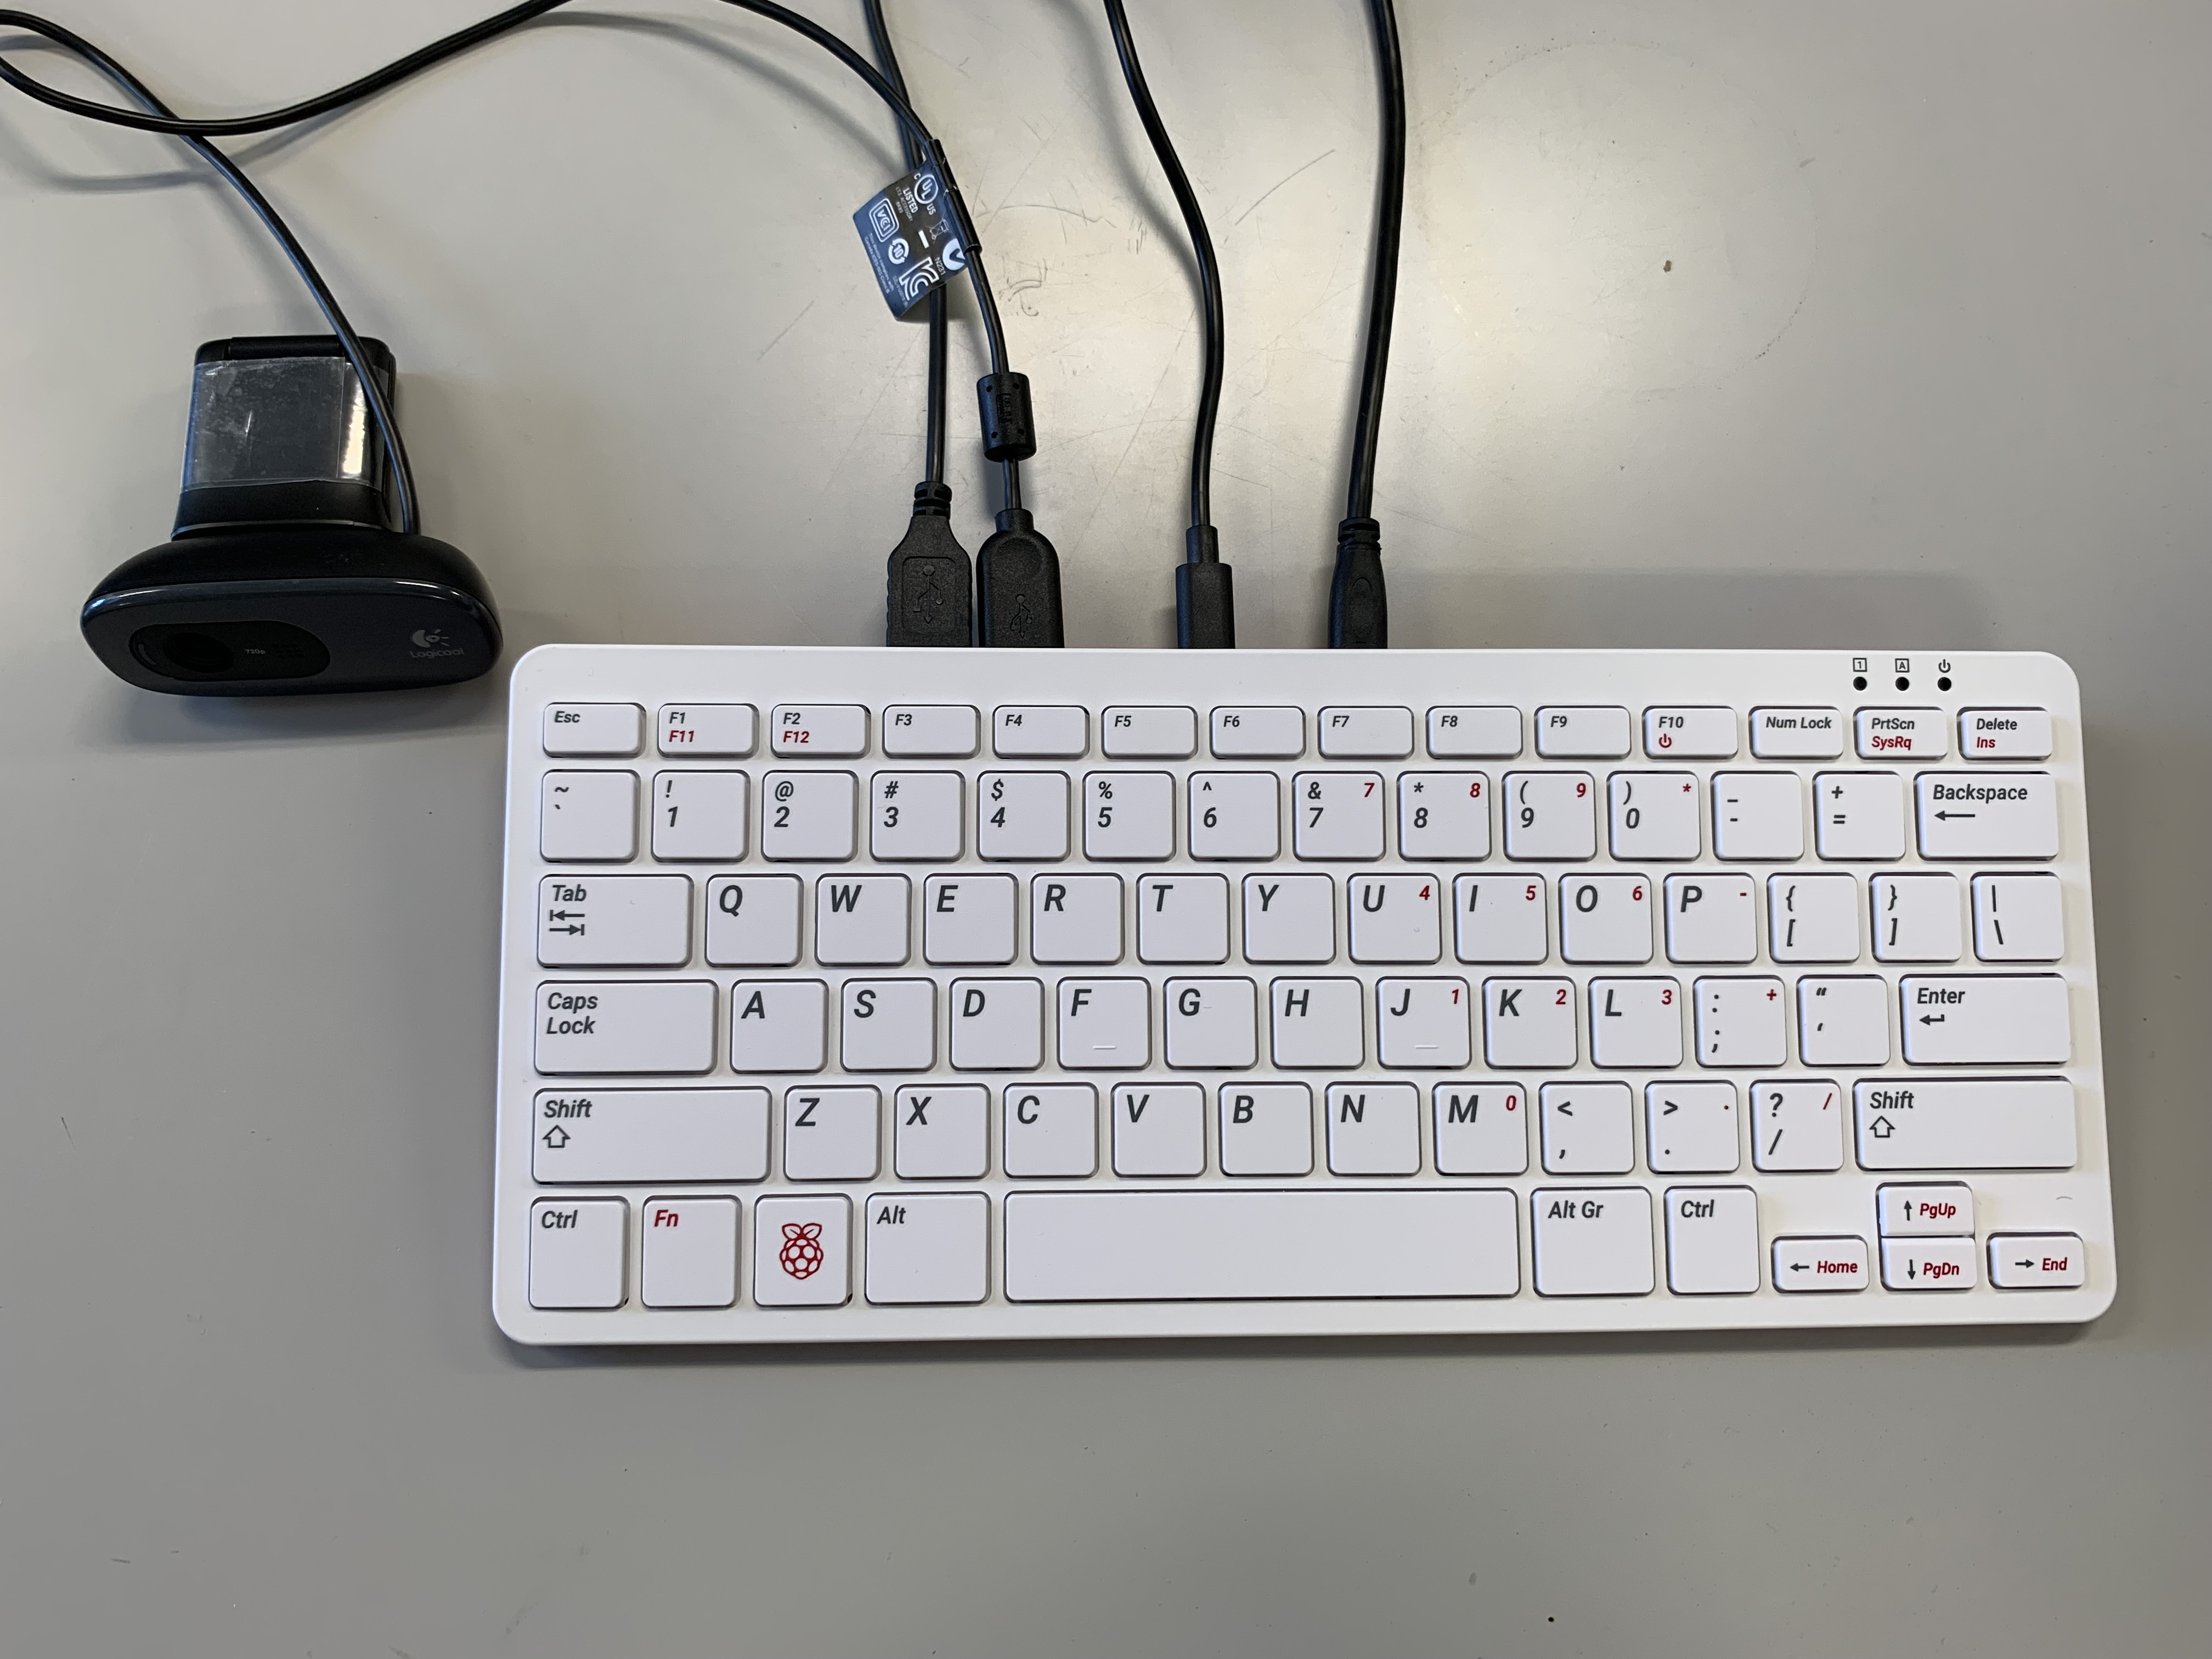
\includegraphics[width=7.904cm]{textbook-img112-2023.jpg}
      \newline
      \stepcounter{Figure}{\theFigure}: Webカメラの接続}
  \end{minipage}
\end{figure}
ウェブカメラを接続したら、ラズベリーパイからウェブカメラの画像を取得してみましょう。左上のラズベリーのアイコンをクリックします。そこから、サウンドとメディアを選択しVLCメディアプレーヤーをクリックします。

\begin{figure}[hb]
  \centering
  \begin{minipage}{10.917cm}
    {\upshape
      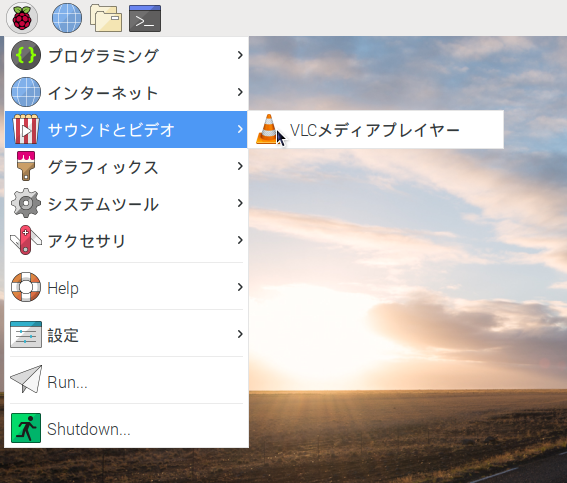
\includegraphics[height=8.715cm]{textbook-img113.png}
      \newline
      \stepcounter{Figure}{\theFigure}: メニューからVLC起動}
  \end{minipage}
\end{figure}
\clearpage
\begin{figure}[ht]
  ~\ref{seq:refFigure20}のようにVLCメディアプレーヤーが起動します。



  \centering
  \begin{minipage}{10cm}
    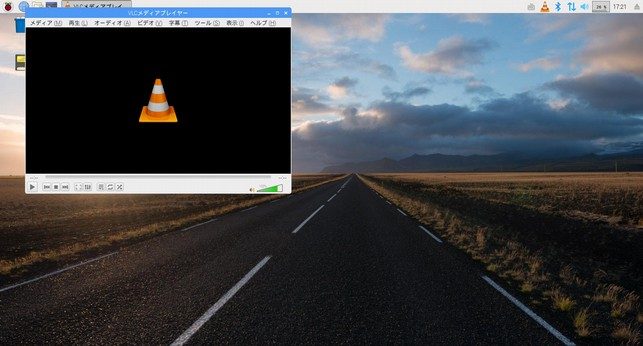
\includegraphics[width=10cm]{textbook-img114.jpg}


    {\refstepcounter{Figure}\theFigure\label{seq:refFigure20}}: VLC起動画面
  \end{minipage}
  \flushleft
  VLCが起動したら確認メッセージが出てきます。

  \textbf{\textcolor[rgb]{1.0,0.2,0.2}{赤わくで囲われているチェックボックスにチェックマーク(\CheckedBox)}}がついていないことを確認して続けるをクリックしてください。



  \centering
  \begin{minipage}{7.186cm}
    {\upshape
      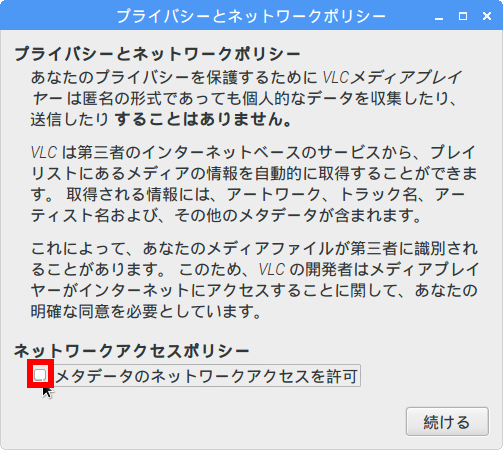
\includegraphics[width=7.2cm]{textbook-img115.png}
      \newline
      \stepcounter{Figure}{\theFigure}: 確認メッセージ}
  \end{minipage}

  \flushleft
  カメラを開きます。~\ref{seq:refFigure22}のように\textbf{メディア}をクリックして\textbf{キャプチャーデバイスを開く}をクリックします。


  \centering
  \begin{minipage}{8.096cm}
    {\upshape
      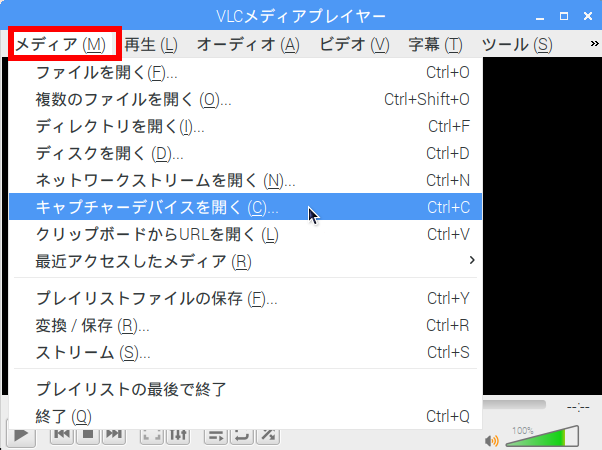
\includegraphics[width=8.0cm]{textbook-img116.png}
      \newline
      {\refstepcounter{Figure}\theFigure\label{seq:refFigure22}}:
      キャプチャデバイスをひらく}
  \end{minipage}
\end{figure}
\clearpage

\begin{figure}[ht]
  ~\ref{seq:refFigure23}のような画面がでてきます。
  赤線で囲われている\textbf{キャプチャーモード}を
  \textbf{Video camera}にして
  青線で囲われている\textbf{再生}をクリックします。


  \centering
  \begin{minipage}{10cm}
    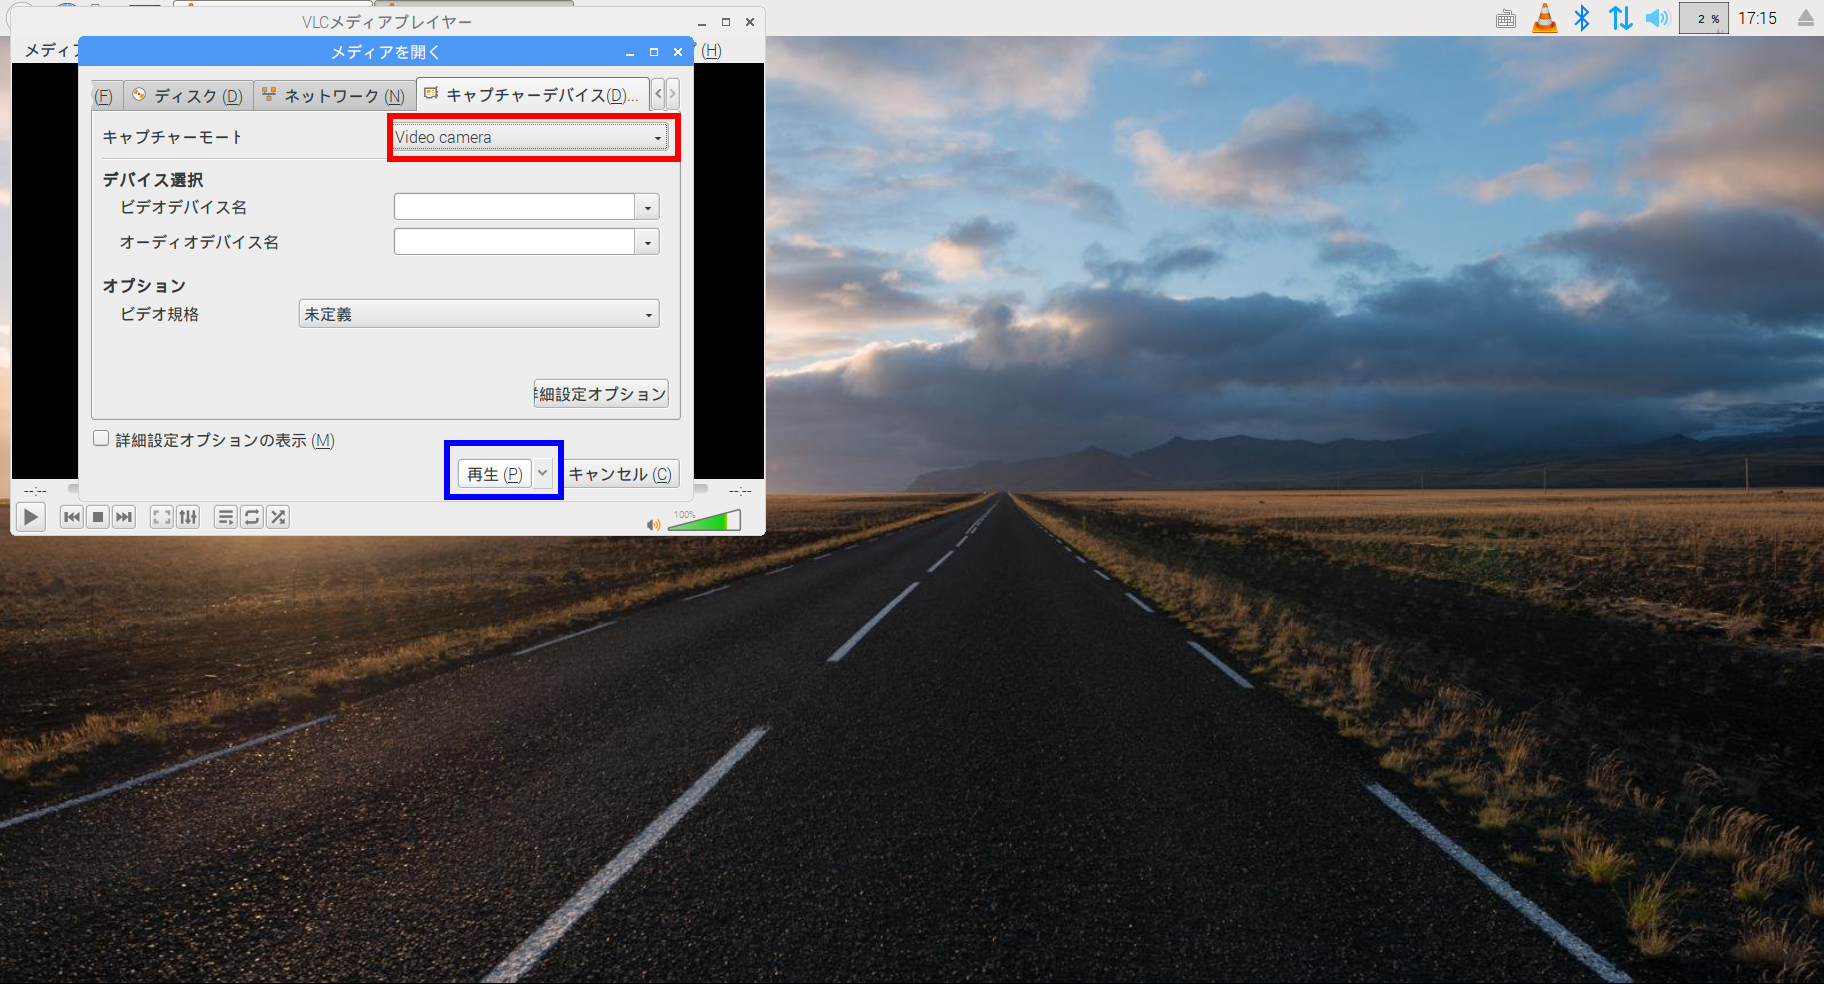
\includegraphics[width=10cm]{textbook-img117.png}
    {\refstepcounter{Figure}\theFigure\label{seq:refFigure23}}:
    キャプチャーデバイスを開く画面
  \end{minipage}

  \flushleft
  しばらくすると、カメラの画像が見えるようになります。

  \centering
  \begin{minipage}{10cm}
    {\upshape
      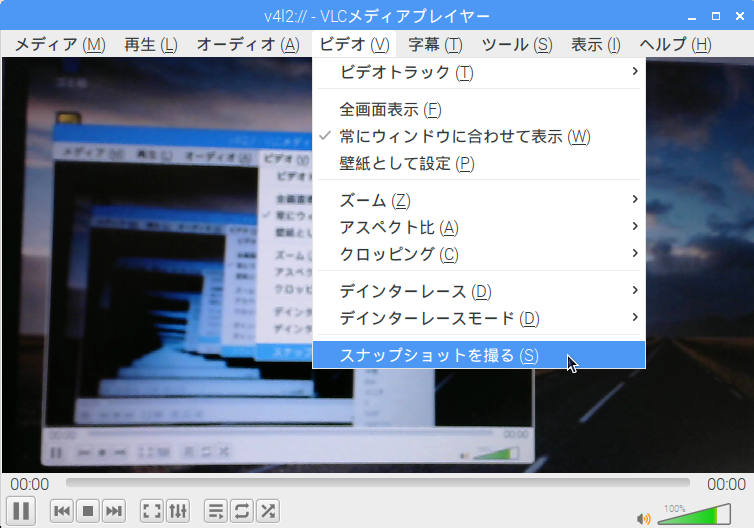
\includegraphics[width=10cm]{textbook-img118.png}
      \newline
      \stepcounter{Figure}{\theFigure}: スナップショット撮影}
  \end{minipage}
  \flushleft

  次に、カメラでさつえいしてみましょう。ビデオをクリックしてスナップショットを撮るをクリックします。


  \centering
  \begin{minipage}{10cm}
    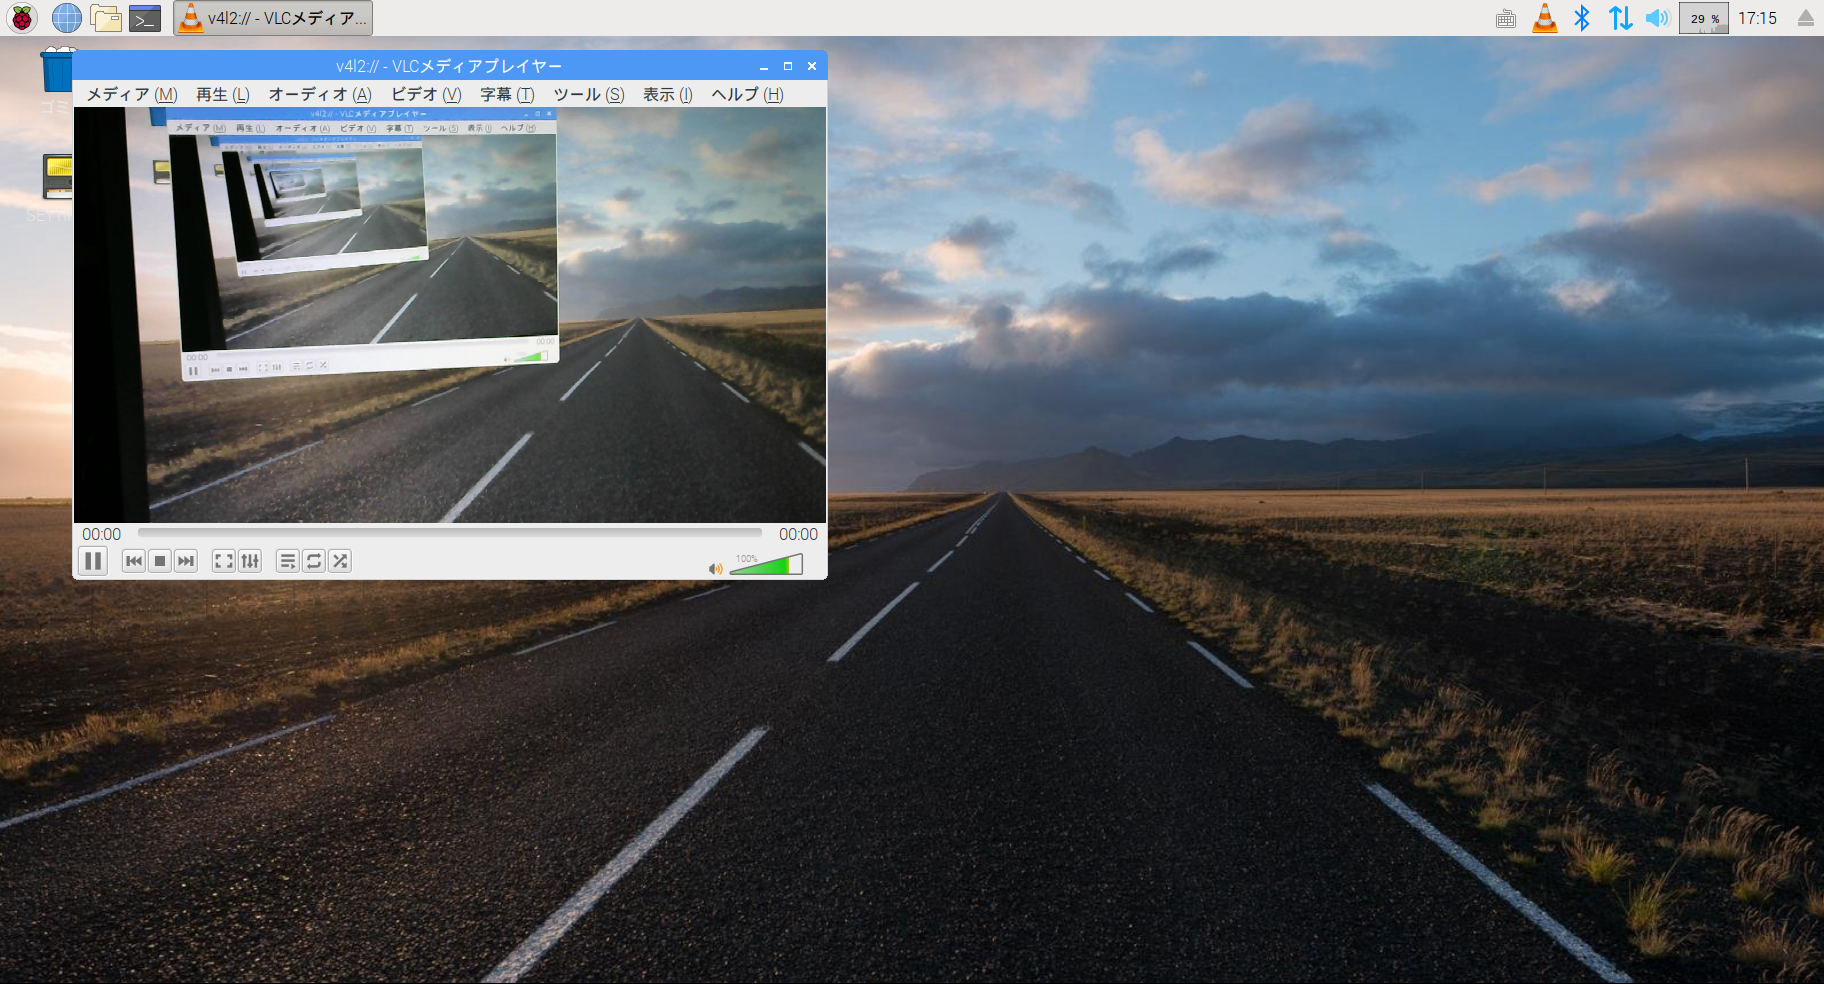
\includegraphics[width=10cm]{textbook-img119.png}
    {\upshape
      \stepcounter{Figure}{\theFigure}: カメラ入力}
  \end{minipage}
\end{figure}
\clearpage
\begin{figure}
  黒線の四角に囲われたように保存場所が表示され、そこへ画像が保存されます。

  \centering
  \begin{minipage}{10cm}
    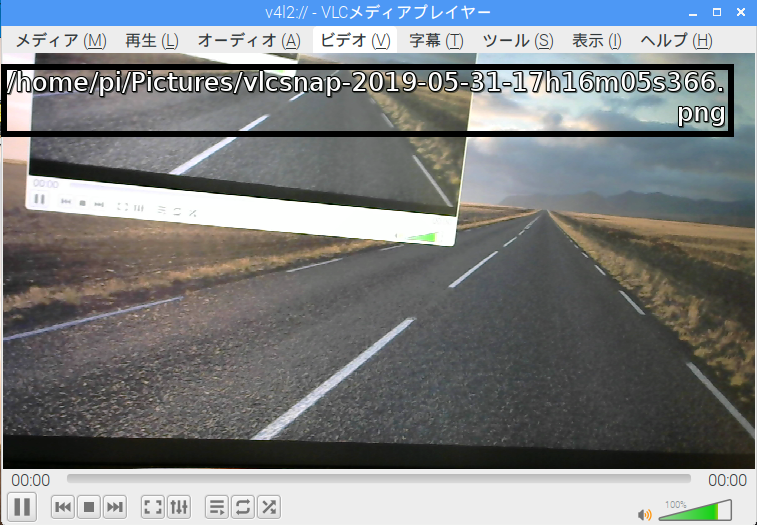
\includegraphics[width=10cm]{textbook-img120.png}
    \stepcounter{Figure}{\theFigure}: スナップショット保存
  \end{minipage}



  \bigskip
  \flushleft

  初期状態ではPicturesの下に保存されます。確認してみましょう。



  \centering
  \begin{minipage}{10cm}
    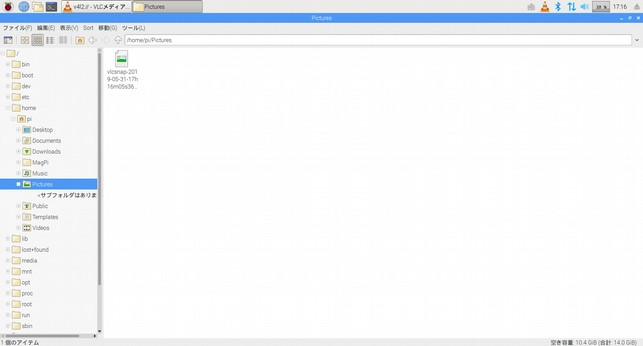
\includegraphics[width=10cm]{textbook-img121.jpg}

    \stepcounter{Figure}{\theFigure}: 画像撮影場所
  \end{minipage}


  \bigskip

  \flushleft
  とった画像を確認してみましょう。~\ref{seq:refFigure28}の赤わくで囲ってあるものがとった写真です。ダブルクリックをすると、画像を開いて見ることができます。



  \centering
  \begin{minipage}{10cm}
    {\upshape
      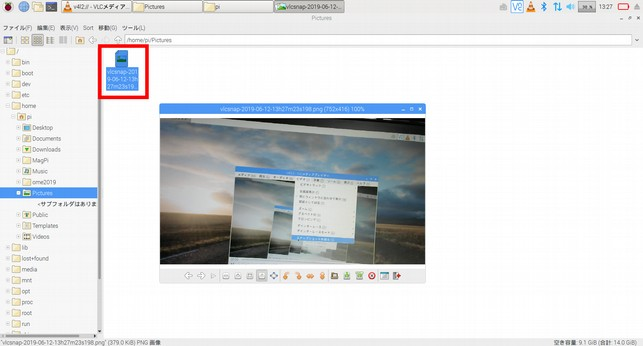
\includegraphics[width=10cm]{textbook-img122.jpg}
      \newline
      {\refstepcounter{Figure}\theFigure\label{seq:refFigure28}}:
      とった画像を開く}
  \end{minipage}
\end{figure}

\bigskip

\clearpage

\begin{figure}[ht]
  \refstepcounter{Exercise}
  \subsection{\theExercise 画像に絵をかこう}

  \bigskip

  “GIMP”ソフトを立ち上げて、色付きの筆で自分の顔写真に絵をかこう

  画像を開いて、色を選択、お絵かきツールの筆を選んで書くよ

  \textbf{考え方}



  \begin{minipage}{\textwidth}
    \centering
    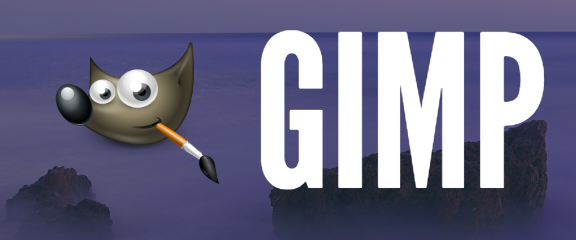
\includegraphics[width=6.112cm]{textbook-img123.png}
    \begin{minipage}[b]{8.617cm}

      本格的な画像編集、加工ソフトの

      GIMPを使って自分の顔写真などの

      画像を編集してみよう
    \end{minipage}


  \end{minipage}
  \bigskip




  \begin{minipage}{\textwidth}
    \centering
    \begin{minipage}{5.852cm}
      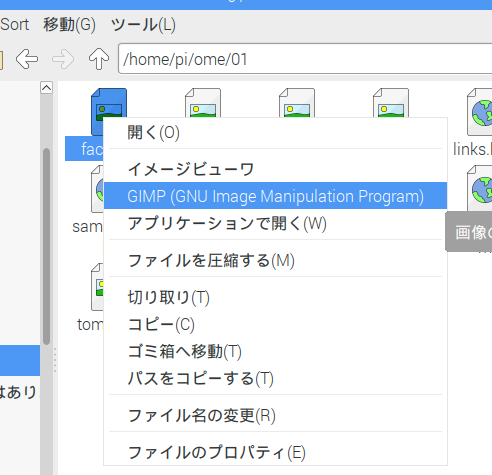
\includegraphics[width=5.359cm]{textbook-img124.png}\\
      1 編集したい画像ファイルを

      右クリックしGIMPをクリック
    \end{minipage}
    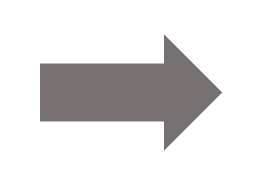
\includegraphics[width=1.489cm]{textbook-img128.png}
    \begin{minipage}{7.975cm}
      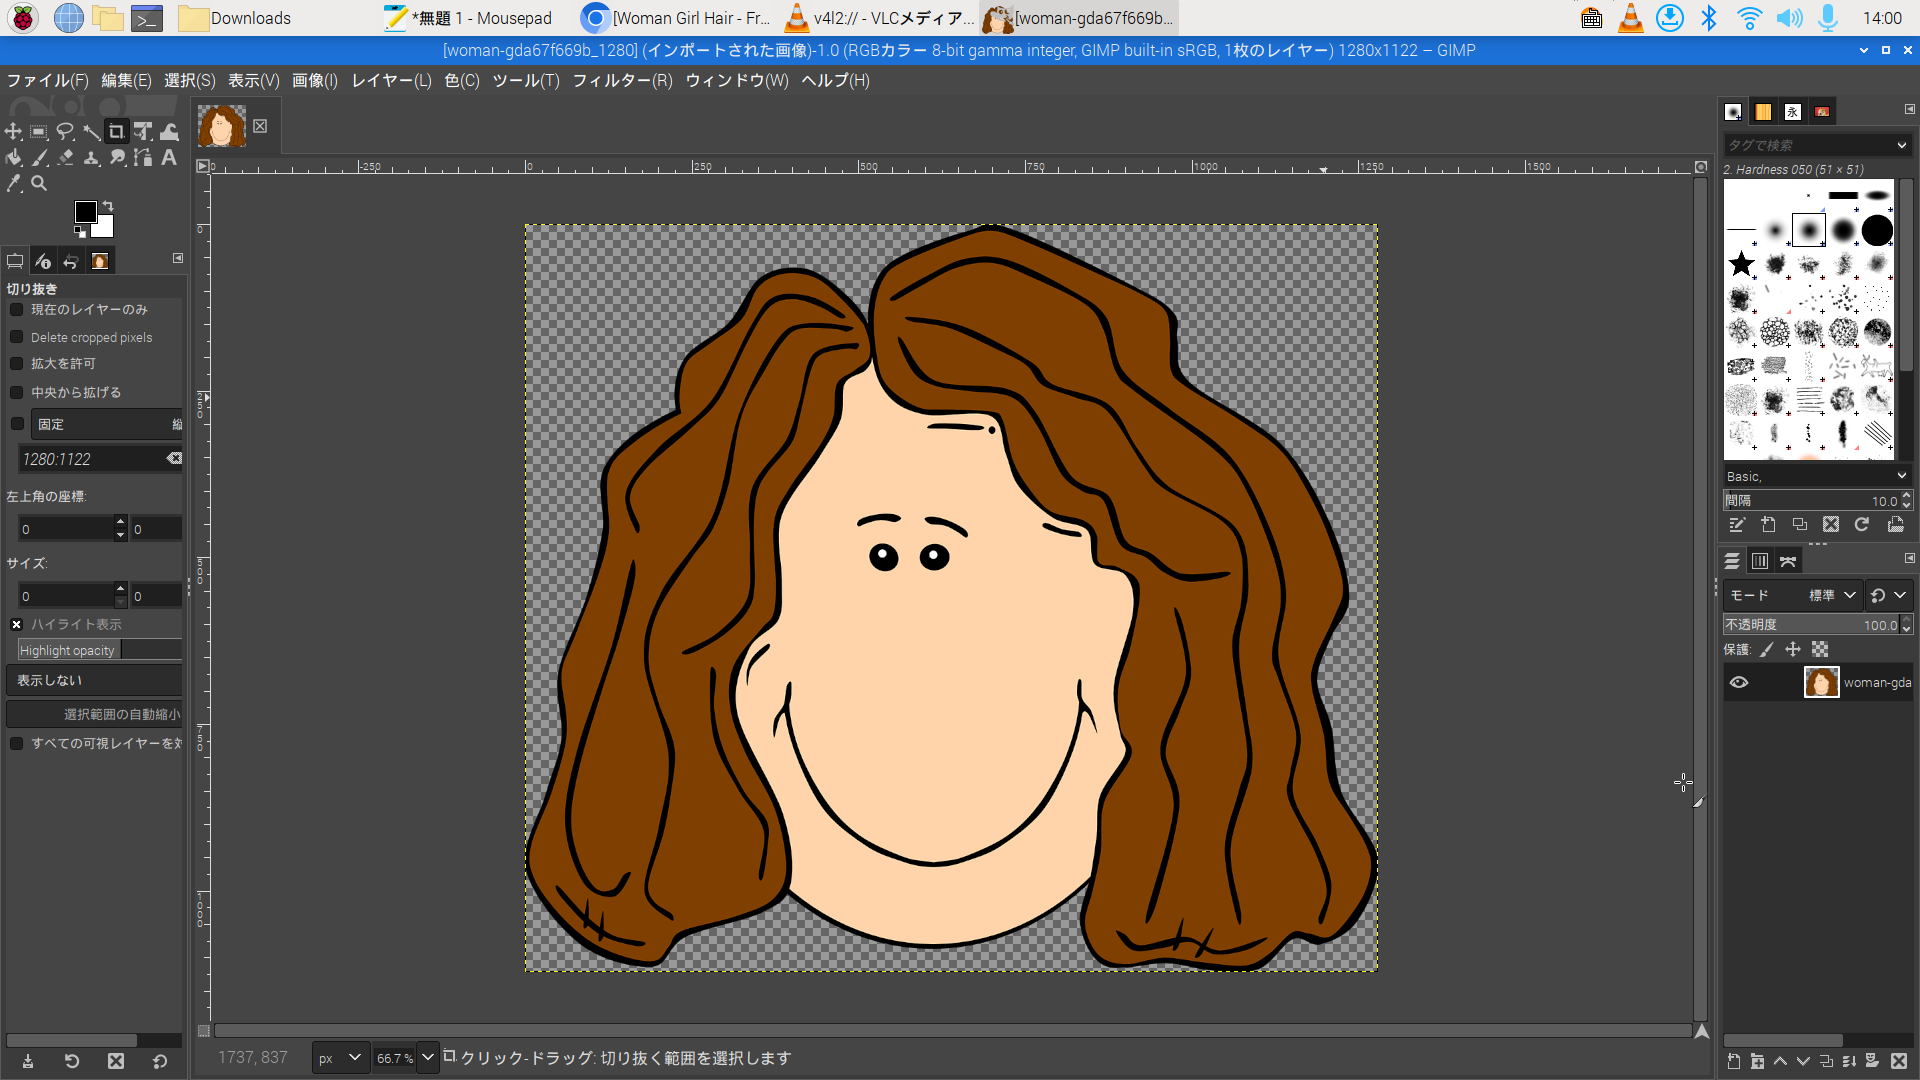
\includegraphics[width=7cm]{textbook-img125.png}\\
      2 画像編集モードになるよ
    \end{minipage}


  \end{minipage}
  \bigskip




  \begin{minipage}{\textwidth}
    \begin{minipage}{5.984cm}
      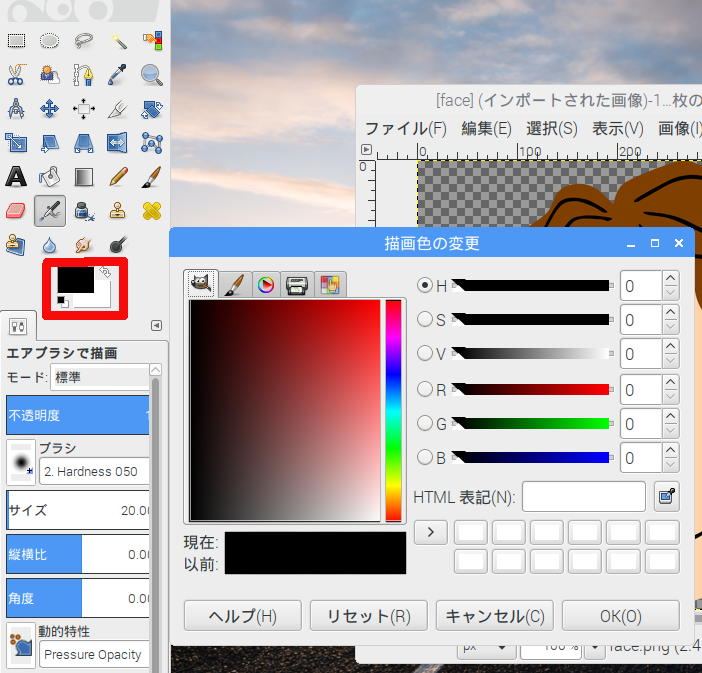
\includegraphics[width=5.971cm]{textbook-img129.png}\\
      3 赤い丸で囲まれている

      部分をクリック


      \bigskip
    \end{minipage}
    \hfill
    \begin{minipage}{8.984cm}
      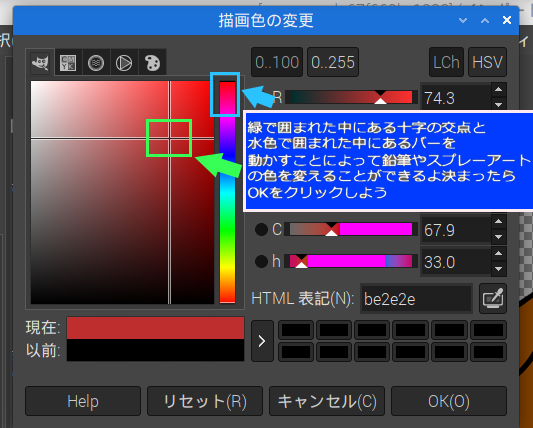
\includegraphics[width=7cm]{textbook-img126.png}\\
      4 色を変更しよう

      好きな色を選んでOKを押します


      \bigskip
      \begin{minipage}{5.984cm}
        5
        今回は色を赤にしました。赤く囲んであるところの色が赤に変わっていることを確認してください。


      \end{minipage}
    \end{minipage}
  \end{minipage}

  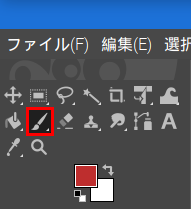
\includegraphics[width=1.866cm]{textbook-img127.png}
  \begin{minipage}[b]{6.663cm}
    6 次にお絵かきツールを選びます。

    赤色で囲われているところをクリックしてください。これで色付きの筆が使えるようになります。


    \bigskip

  \end{minipage}
\end{figure}
\clearpage
\begin{figure}[ht]
  \textbf{考え方(続き)}

  \begin{minipage}{\textwidth}
    \centering
    \begin{minipage}{5.76cm}
      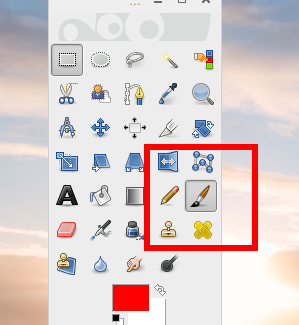
\includegraphics[width=5.05cm]{textbook-img130.png}\\
      7
      ツール一覧の下の文字が「ブラシで描画」に変わったことを確認しましょう。これで筆が使えるようになりました。
    \end{minipage}
    \hfill
    \begin{minipage}{10.2cm}
      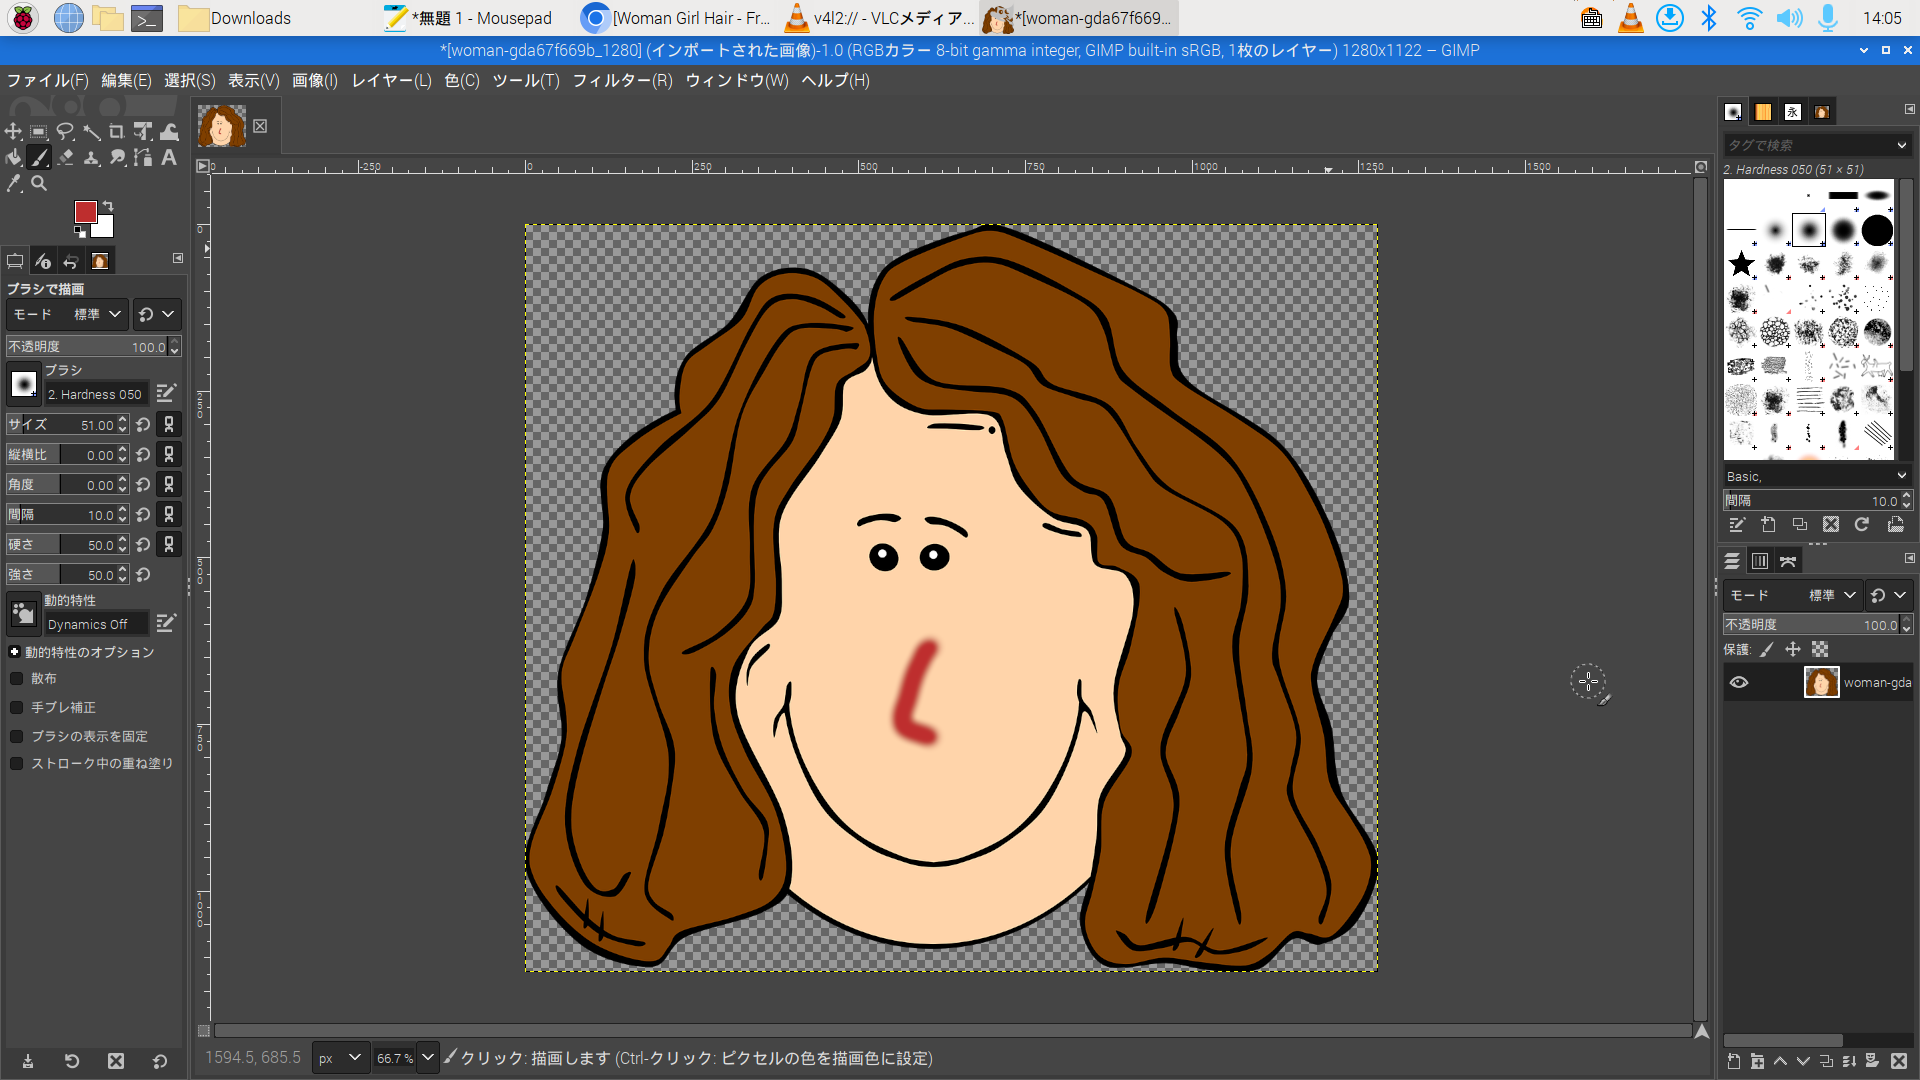
\includegraphics[width=10.134cm]{textbook-img131.png}\\
      8 左クリックをおしながら画像の上を移動させると筆でお絵かきができます。いたずら書きをしてみてください
    \end{minipage}
  \end{minipage}


  \bigskip

  \begin{minipage}{\textwidth}
    \begin{minipage}{6.984cm}
      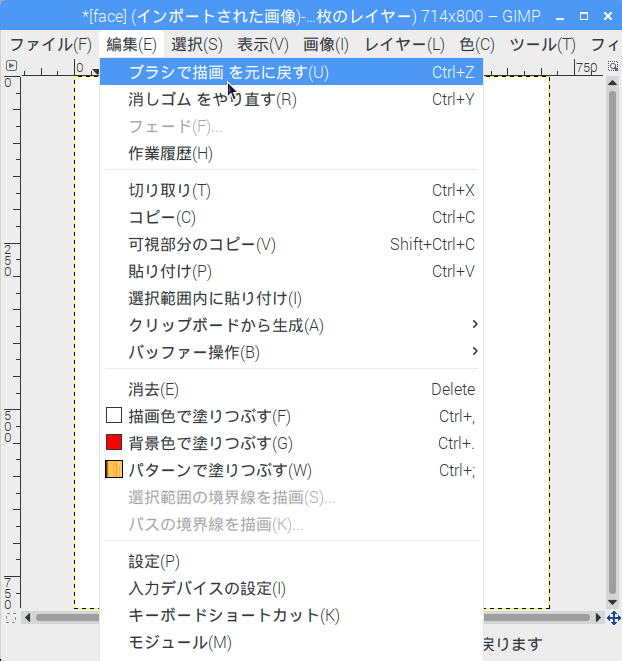
\includegraphics[width=6.228cm]{textbook-img132.png}\\
      9 間違えてしまって、もとに戻したいとなったらメニューの編集からもとに戻すをクリックします。
    \end{minipage}
    \hfill
    \begin{minipage}{8.966cm}
      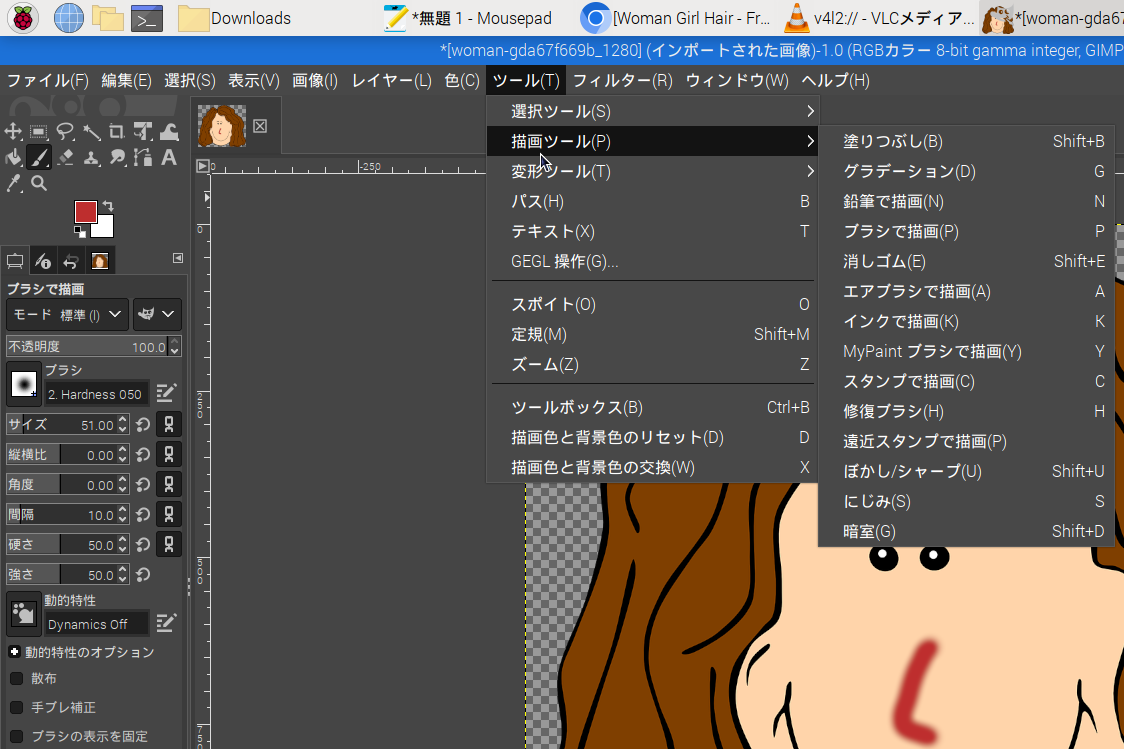
\includegraphics[width=8.881cm,height=4.997cm]{textbook-img133.png}\\
      10 他にもたくさんツールはあります。メニューのツール欄にある描画ツールで選べるよ。鉛筆、インクを試してみよう。書き方はいっしょで左クリックを押しながら移動だよ
    \end{minipage}
  \end{minipage}
\end{figure}


\clearpage
\begin{figure}
  \textbf{考え方(続き)}


  編集しおわったら書き出しをします。

  \centering
  \begin{minipage}{\textwidth}
    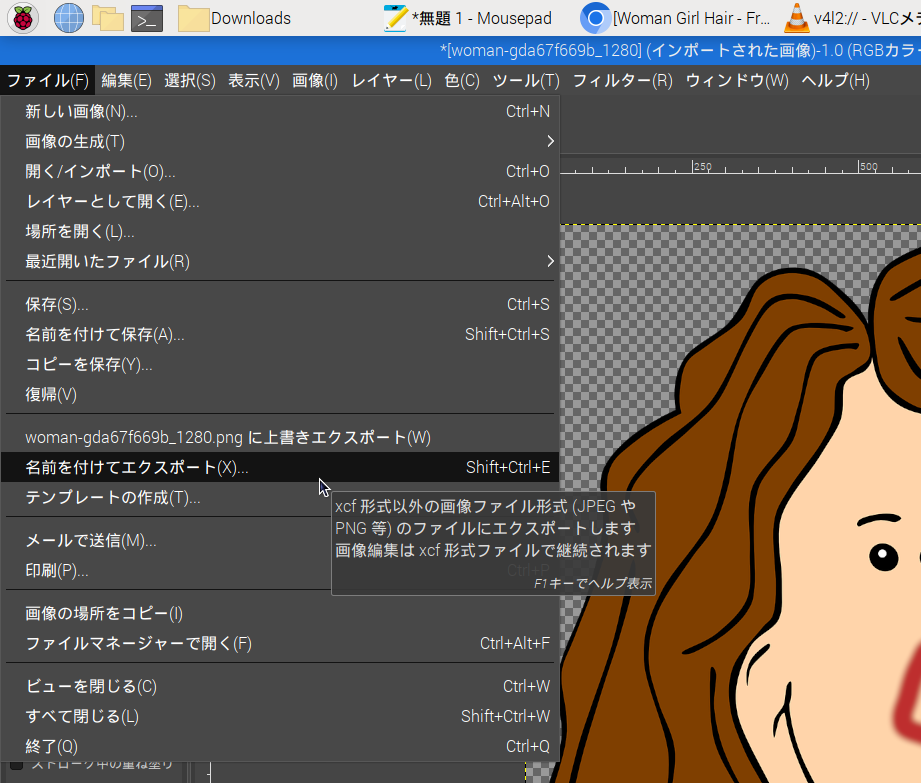
\includegraphics[width=0.5\textwidth]{textbook-img138.png}\\
    11 編集がおわったら

    ファイルから名前を付けてエクスポートをクリック
  \end{minipage}

  \bigskip


  \begin{minipage}{\textwidth}
    \begin{minipage}{7.7cm}
      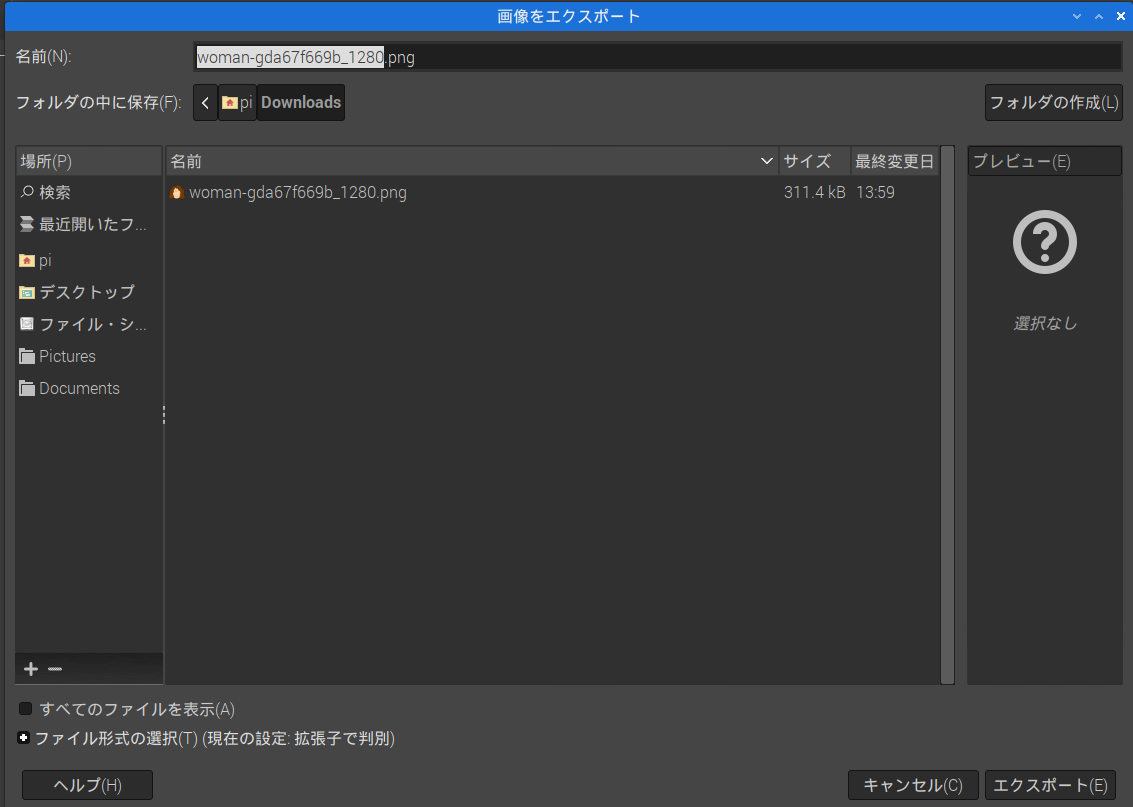
\includegraphics[width=7.615cm]{textbook-img137.png}\\
      12
      下のエクスポートをクリック(.jpegファイルから編集したならば12へ)
    \end{minipage}
    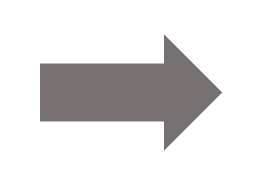
\includegraphics[width=1.919cm]{textbook-img135.png}
    \begin{minipage}{7.786cm}
      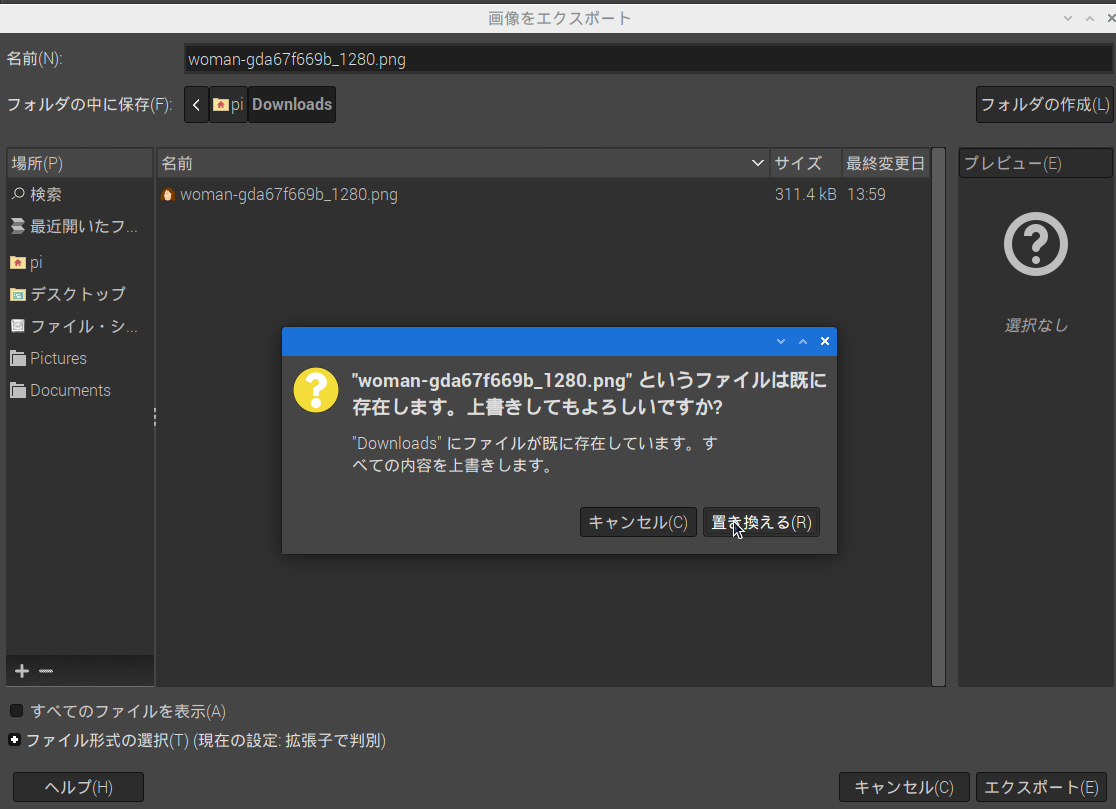
\includegraphics[width=7.352cm]{textbook-img136.png}\\
      13 置き換えるをクリック
    \end{minipage}
  \end{minipage}

  \bigskip


  \begin{minipage}{\textwidth}
    \begin{minipage}{8.074cm}
      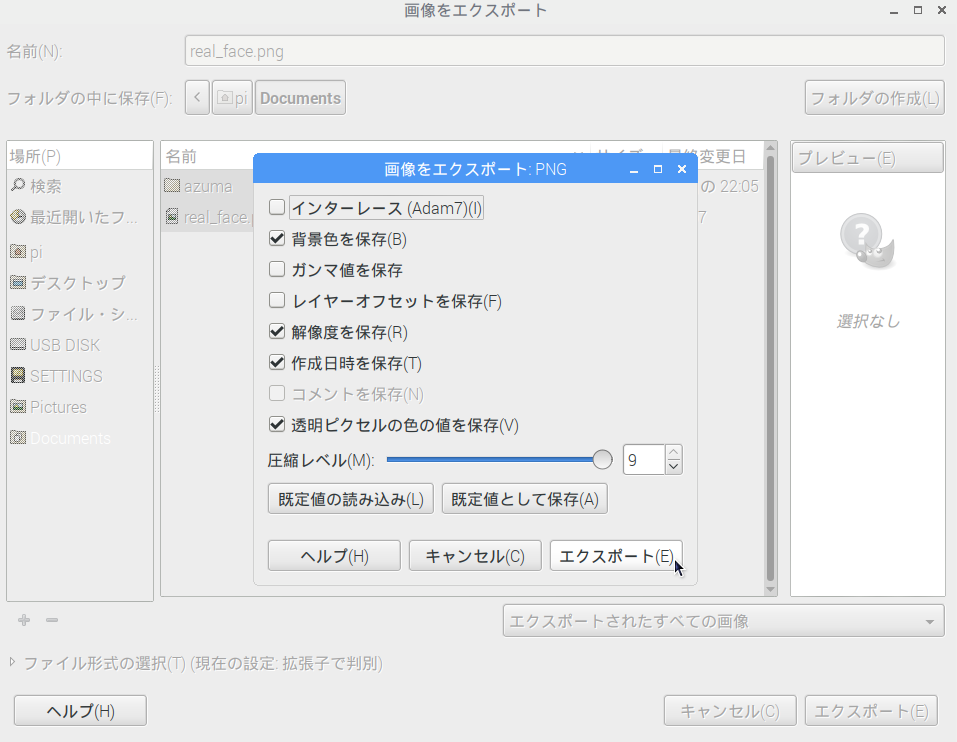
\includegraphics[width=7.721cm]{textbook-img134.png}\\
      14 エクスポートをクリック
    \end{minipage}
    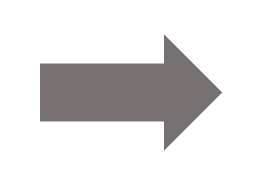
\includegraphics[width=1.919cm]{textbook-img135.png}
    \begin{minipage}{7.328cm}
      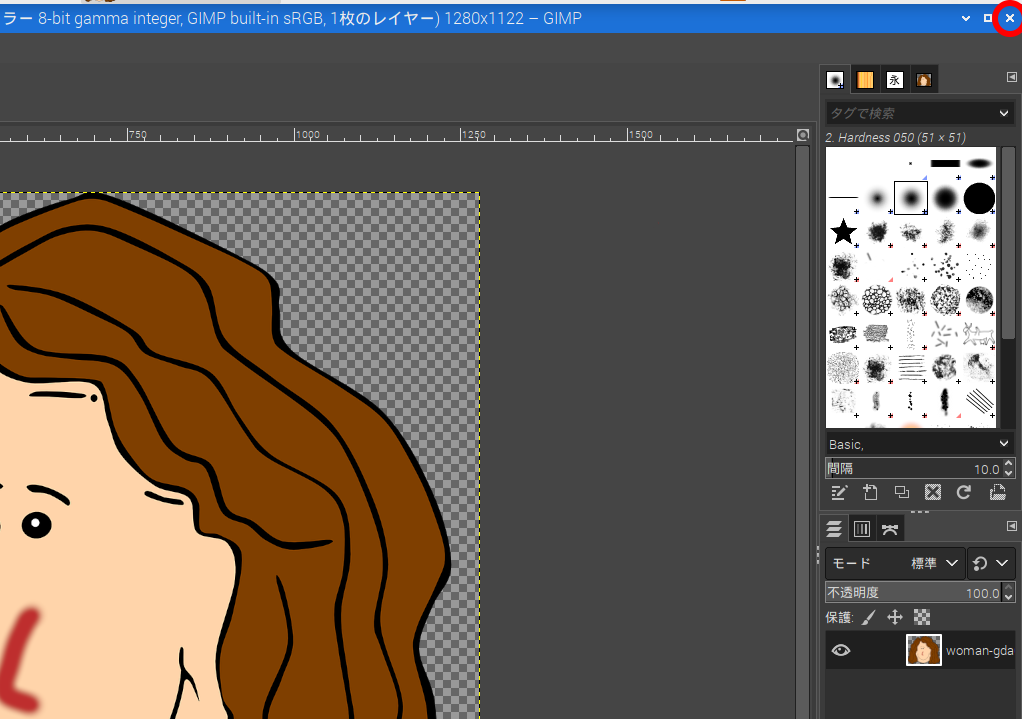
\includegraphics[width=7.061cm]{textbook-img1030.png}\\
      15
      右上の赤い丸で囲まれた×ボタンを押して、画像編集ツールを閉じよう
    \end{minipage}
  \end{minipage}



\end{figure}
\clearpage

\begin{minipage}{0.45\linewidth}
  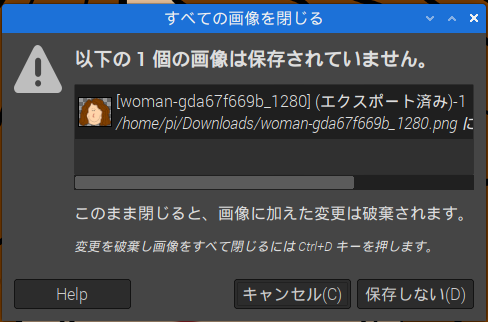
\includegraphics[width=\linewidth,height=5cm]{textbook-img1031.png}\\
  16 「保存されていません」というウィンドウがでます。これは、先ほど「エクスポート」したものとは別のことを言っていて、
  画像自体は保存されています。なので、気にせず「保存しない」をクリックしましょう
\end{minipage}
\hfill
\vspace{20pt}
\begin{minipage}{0.45\linewidth}
  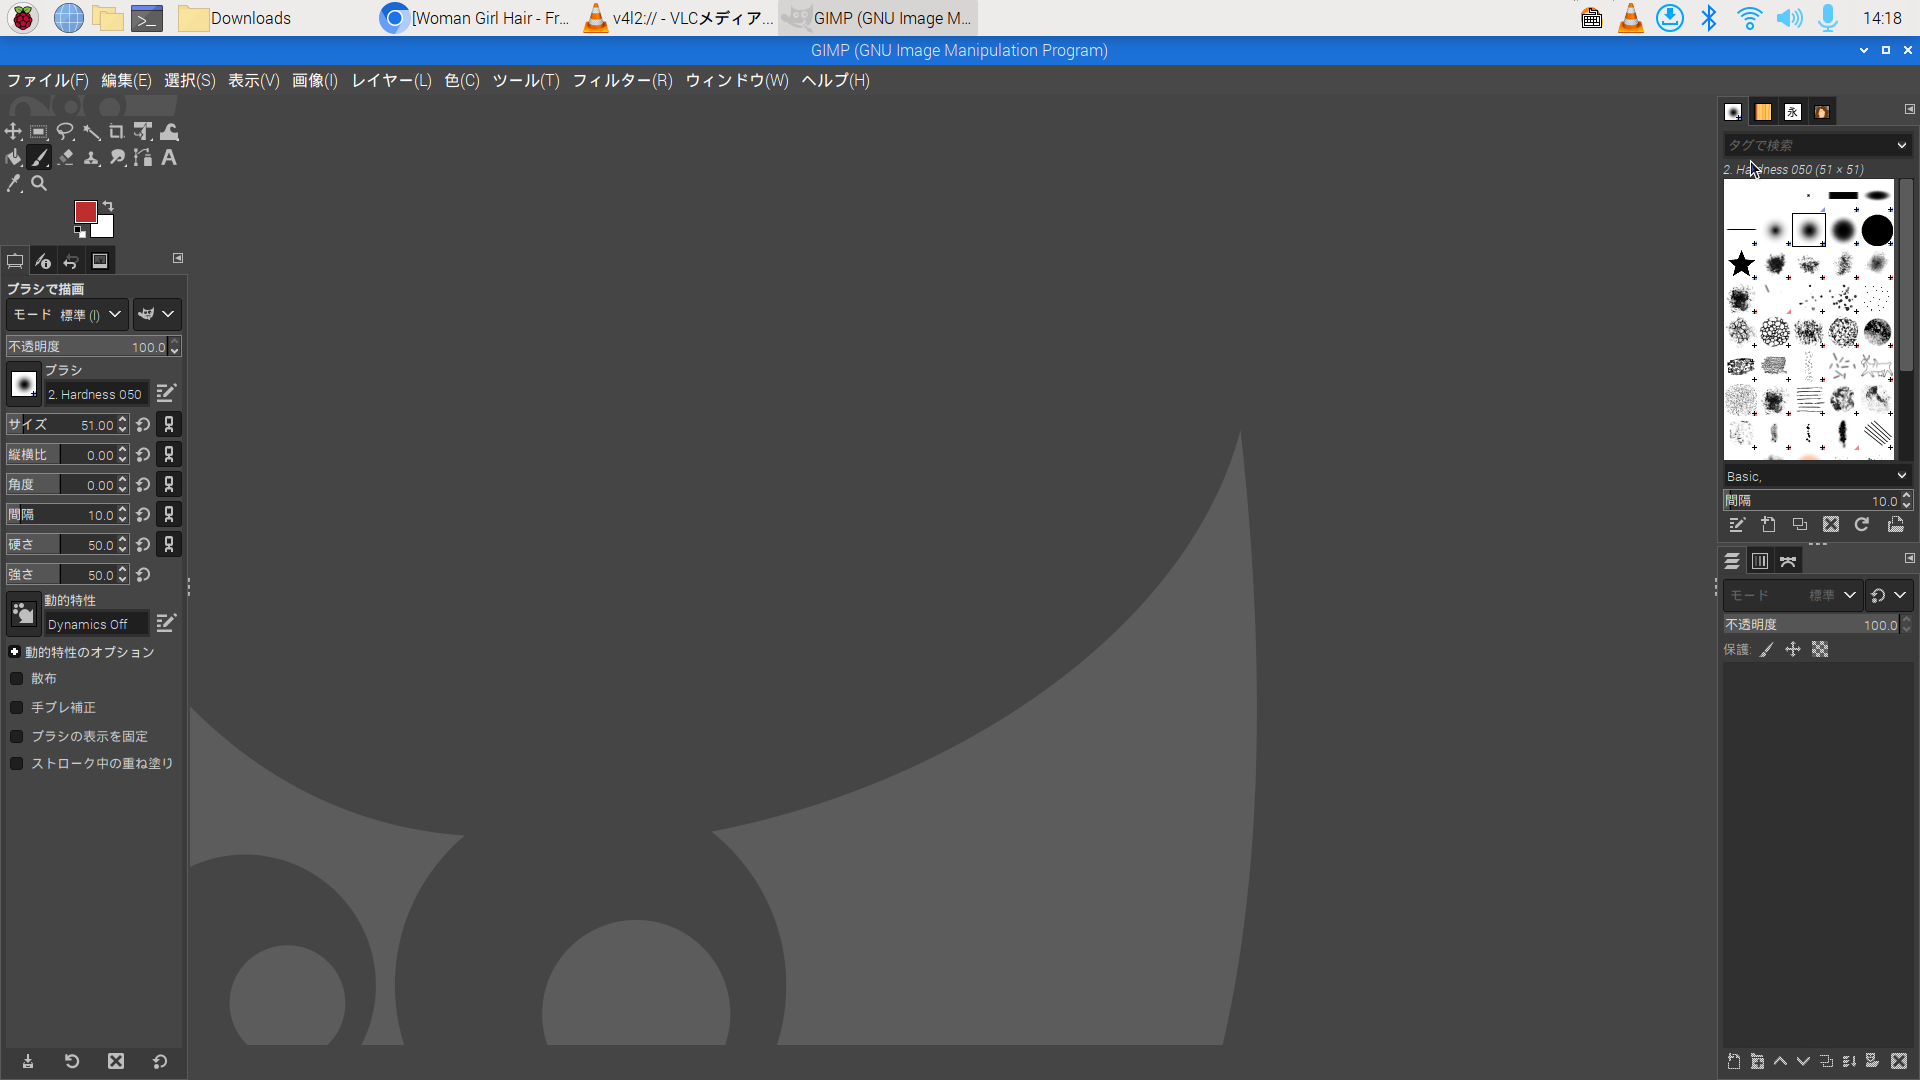
\includegraphics[width=\linewidth,height=5cm]{textbook-img1032.png}\\
  17 画像が消え、何もないウィンドウになります。右上の×ボタンをクリックして、画像編集ツールを閉じましょう
\end{minipage}
\begin{minipage}{0.45\linewidth}
  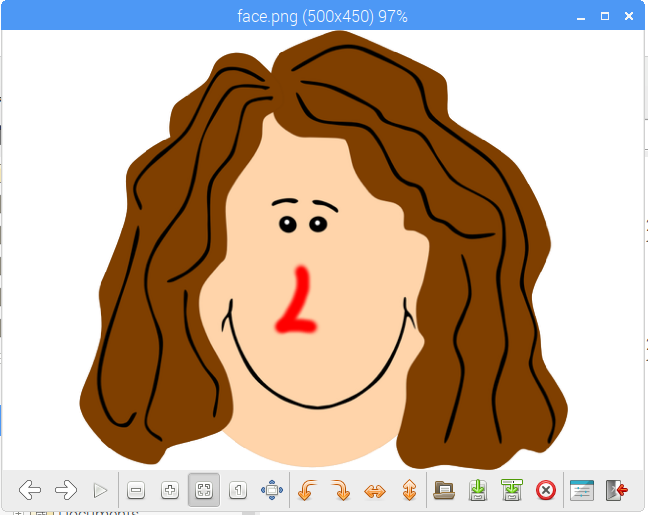
\includegraphics[width=\linewidth,height=5cm]{textbook-img139.png}\\
  18 画像ファイルを開いて確認してみよう
\end{minipage}
\hfill
\vspace{20pt}

\refstepcounter{Question}\theQuestion

”GIMP”を使って、自分の顔写真をさらに編集、加工してみよう

\begin{figure}[ht]
  \centering
  \begin{minipage}{9.082cm}
    {\upshape
      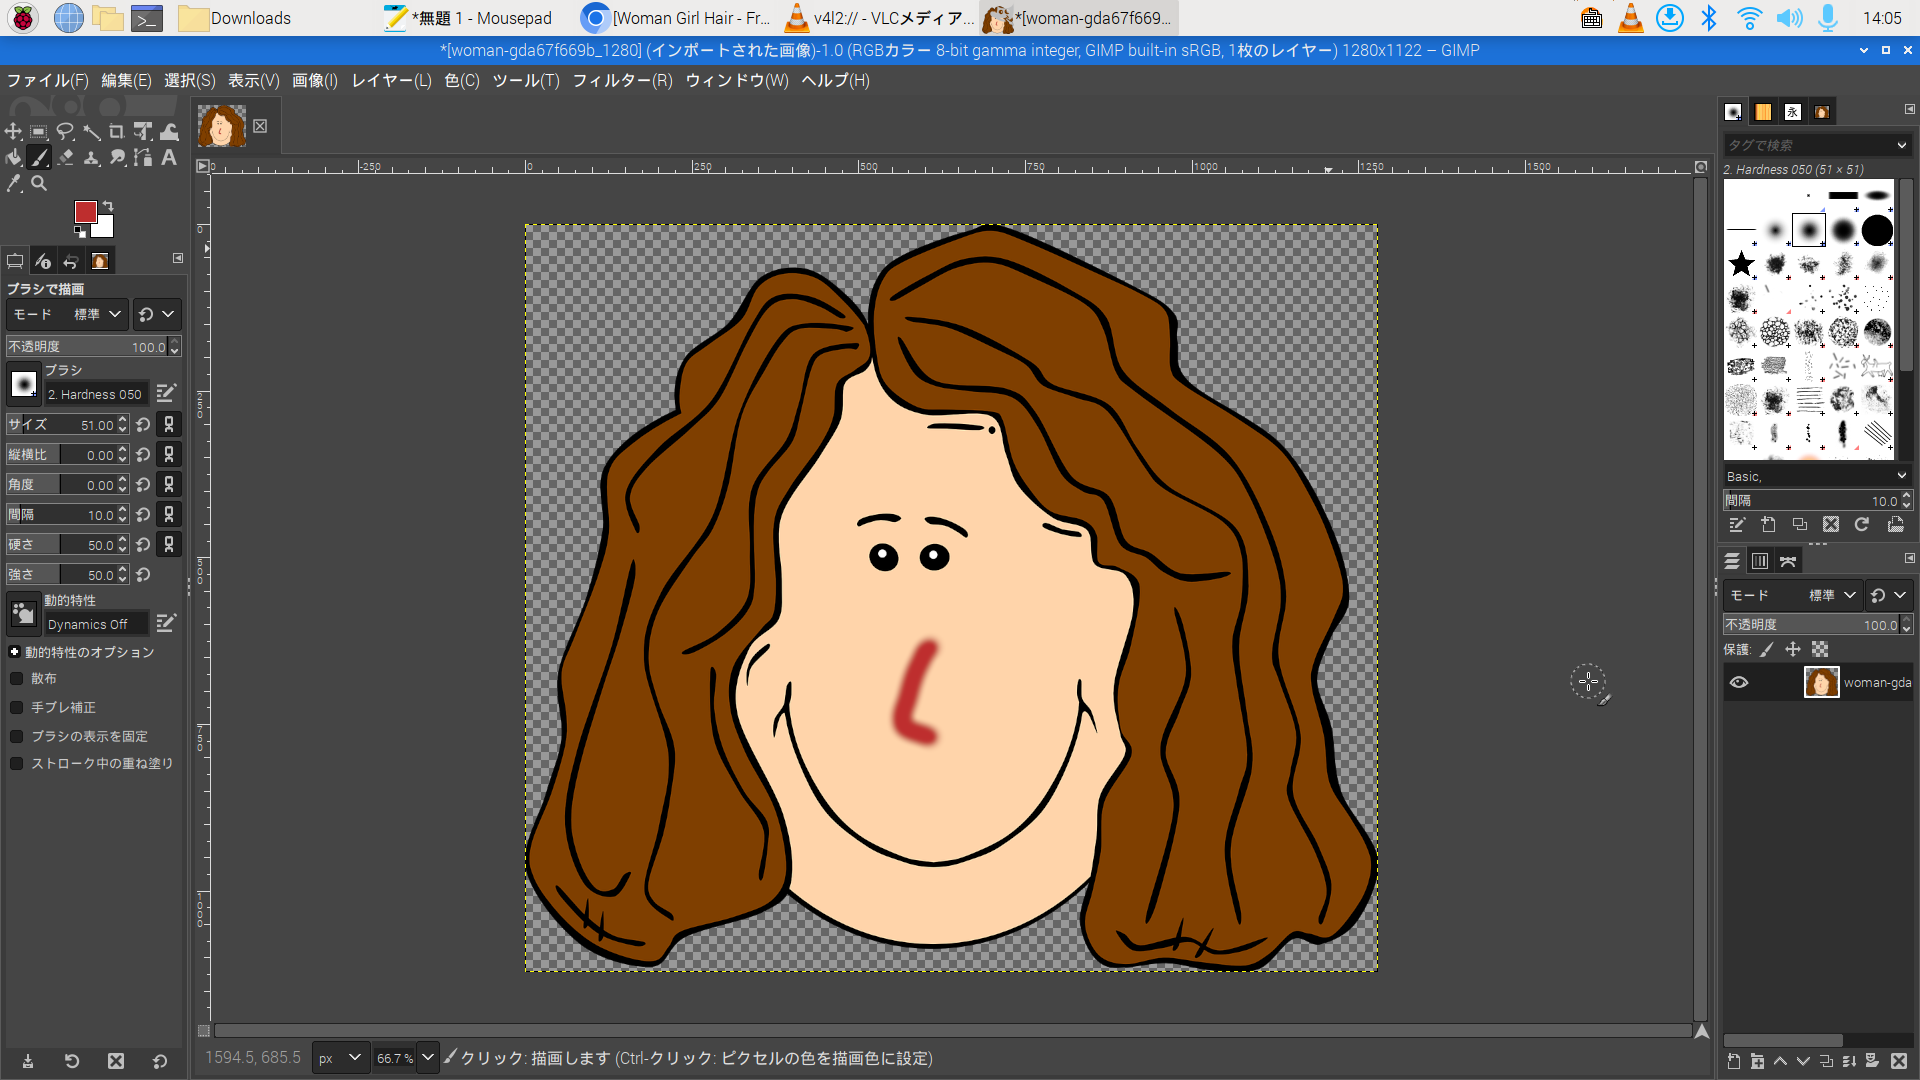
\includegraphics[width=9.082cm]{textbook-img131.png}
      \newline
      \stepcounter{Figure}{\theFigure}: GIMP画像編集}
  \end{minipage}
\end{figure}


\clearpage
\end{document}
